\subsection{Attributive Language with Complement
($\ALC$)}\label{attributive-language-with-complement-alc}

\subsubsection{Konzept- und Rollennamen}\label{konzept--und-rollennamen}

Konzept- und Rollennamen sind abzählbar unendliche und disjunkte (durch Groß- und Kleinschreibung) Mengen.

\subsubsection{$\ALC$: Syntax}\label{alcsyntax}

\theoremstyle{definition}
\begin{definition}{$\ALC$-Konzepte} \\
  Die Menge der $\ALC$-Konzepte is induktiv definiert:
  \begin{itemize}
    \item Jeder Konzeptname ist $\ALC$-Konzept
    \item Wenn $C$, $D$ $\ALC$-Konzepte, so auch
    \begin{itemize}
      \item $\neg C$ \tabto{2cm}(Negation)
      \item $C \sqcap D$ \tabto{2cm}(Konjunktion)
      \item $C \sqcup D$ \tabto{2cm}(Disjunktion)
    \end{itemize}
    \item {Wenn $C$ $\ALC$-Konzept und $r$ Rollenname, so sind
    \begin{itemize}
      \item $\exists r.C$ \tabto{2cm}(Existenzrestriktion)
      \item $\forall r.C$ \tabto{2cm}(Werterestriktion)
    \end{itemize}
    $\ALC$-Konzepte}
  \end{itemize}
\end{definition}

\textbf{T2.1 Beispiel}

Hier einige Beispiel für diese Syntax:

\begin{center}
$Student \sqcap \exists studiert.Naturwissenschaft$ \\
$Professor \sqcap Emeritus \sqcap \forall haelt.\neg PlichtVL$ \\
$VL \sqcap \neg PlichtVL \sqcap \forall hatUebungsaufgabe(Einfach \sqcup Interessant)$ \\
$A \sqcap \exists r.(\neg B \sqcup \forall r.A)$
\end{center}

\textbf{Weiteres zur Syntax}

Dabei verwenden wir folgende Symbole:

\begin{itemize}
  \item{$A$,$B$ für Konzeptnamen}
  \item{$C$,$D$ für zusammengesetzte Konzepte}
  \item{$r$,$s$ für Rollennamen}
\end{itemize}

Zudem benutzen zudem folgende Abkürzungen: wir schreiben

\begin{itemize}
  \item{$\top$ für $A \sqcup \neg A$}
  \item{$\bot$ für $A \sqcap \neg A$}
\end{itemize}

\textbf{Präzedenzregel}

\begin{itemize}
  \item{$\neg$,$\exists$,$\forall$ binden stärker als $\sqcap$ und $\sqcup$}
\end{itemize}

Also zum Beispiel steht $\forall r.(\exists r.A \sqcap B)$ für $\forall r.((\exists r.A) \sqcap B)$ und nicht für $\forall r.(\exists r.(A \sqcap B))$.

Desweiteren is keine Präzedenz zwischen $\sqcap$ und $\sqcup$ definiert worden: Daher müssen Klammern verwendet werden!

\subsubsection{$\ALC$: Semantik}

\begin{definition}{$\ALC$ Semantik} \\
Eine \emph{Interpretation} $\MI$ ist Paar ($\Delta^{\MI}$,$\cdot^{\MI}$) mit
  \begin{itemize}
    \item{$\Delta^{\MI}$ nicht leere Menge (\emph{Domäne})}
    \item{$\cdot^{\MI}$ \emph{Interpretationsfunktion} bildet ab:
     \begin{itemize}
       \item{jeden Konzeptnamen $A$ auf Menge $A^{\MI} \subseteq \Delta^{\MI}$}
       \item{jeden Rollennamen $r$ auf Relation $r^{\MI} \subseteq \Delta^{\MI} \times \Delta^{\MI}$}
     \end{itemize}}
  \end{itemize}
\end{definition}

\noindent Abbildung $\cdot^{\MI}$ wird induktiv auf zusammengesetzte Konzepte erweitert:

\begin{itemize}
  \item $(\neg C)^{\MI} = \Delta^{\MI} \setminus C^{\MI}$
  \item $(C \sqcap D)^{\MI} = C^{\MI} \cap D^{\MI}$
  \item $(C \sqcup D)^{\MI} = C^{\MI} \cup D^{\MI}$
  \item $(\exists r.C)^{\MI} = \{d \in \Delta^{\MI} |$ es gibt $ e \in \Delta^{\MI}$ mit $(d,e) \in r^{\MI}$ und $e \in C^{\MI}\}$
  \item $(\forall r.C)^{\MI} = \{d \in \Delta^{\MI} |$ für alle $ e \in \Delta^{\MI}$, $(d,e) \in r^{\MI}$ impliziert $e \in C^{\MI}\}$
\end{itemize}

Verwendete Simbole:

\begin{itemize}
  \item $\MI$, $\MJ$ für Interpretationen
  \item $d$, $e$ für Elemente der Domäne
\end{itemize}

Für Interpretationen verwenden wir übliche Terminologie für Graphen:

\begin{itemize}
  \item $e$ für $r$-Nachfolger von $d$ (in $\MI$) wenn ($d$, $e$) $\in r^{\MI}$
  \item $e$ für $r$-Vorgänger von $d$ (in $\MI$) wenn ($e$, $d$) $\in r^{\MI}$
  \item wenn $r$ unwichtig, sprechen wir nun von Nachfolgern / Vorgängern
  \item $\MI$ ist endlich gdw. $\Delta^{\MI}$ endlich ist.
\end{itemize}

\subsubsection{Extension/Modell}\label{exetension}

Wir nennen

\begin{itemize}
\item
  $C^{\MI}$ ist \emph{Extension} des Konzeptes oder der Rolle $C$
\item
  jedes $d \in C^{\MI}$ ist eine Instanz des Konzeptes $C$
\item
  $r$-Nachfolger, $r$-Vorgänger
\end{itemize}

Beachte, das $\top^{\MI}$ für jede Interpretation $\MI$ identisch mit $\Delta^{\MI}$ ist. Intuitivt entspricht $\top$ die Menge alle Elemente. 

$\bot^{\MI}$ ist für jede Interpretation $\MI$ leer, repräsentiert also intuitiv, dass etwas unmöglich ist. Z.B.:

Mensch $\sqcap$ $\forall$hatKind.$\bot$
Menschen, die keine Kinder haben

{\subsubsection{Erfüllbarkeit,Subsumtion,Äquivalenz}\label{erfuxfcllbarkeit-subsumtion-uxe4quivalenz}}

\begin{definition}{Erfüllbar, susumiert, äquivalent} \\
Seien $C$ und $D$ $\ALC$-Konzepte. Dann

\begin{itemize}
\item
  ist $C$ \emph{erfüllbar}, wenn es eine Interpretation $\MI$ gibt mit
  $C^{\MI} \neq \varnothing$. $\MI$ ist dann ein \emph{Modell} von
  $C$.
\item
  wird $C$ von $D$ \emph{subsumiert}, wenn $C^{\MI} \subseteq D^{\MI}$
  in allen Interpretationen $\MI$ (Notation $C \sqsubseteq D$)
\item
  sind C und D \emph{äquivalent}, wenn $C^{\MI} = D^{\MI}$ in allen
  Interpretationen $\MI$ (Notation $C \equiv D$)
\end{itemize}
\end{definition}

Es gelten die üblichen aussagenlogischen Äquivalenten, wie z.B. de
Morgan.

\subsection{TBoxen}\label{tboxen}

TBoxen definieren Konzepte und setzten diese zueinander in Beziehung.

\subsubsection{TBox-Syntax}\label{tboxsyntax}

\begin{definition}{TBox-Syntax} \\
\emph{Konzeptinklusion} ist Ausdruck $C \sqsubseteq D$ mit $C$, $D$ Konzepten. \\
\emph{TBox} ist endliche Menge von Konzeptinklusionen. \\
Wir verwenden $C \equiv D$ als Abkürzung für $C \sqsubseteq D$, $D \sqsubseteq C$. 

Wir lesen $C \equiv D$ als ``$C$ impliziert $D$''.
\end{definition}

\subsubsection{TBox-Sematik}\label{tboxsemantik}

\begin{definition}{TBox-Semantik} \\
Eine Interpretation $\MI$
\begin{itemize}
\item
  erfüllt Konzeptinklusion $C \sqsubseteq D$ gdw.
  $C^{\MI} \subseteq D^{\MI}$
\item
  ist Modell von TBox $\MT$ gdw. $\MI$ alle Konzeptinklusionen in $\MT$
  erfüllt
\end{itemize}
\end{definition}

Intuitiv entsprechen Interpretation mögliche Welten, TBoxen hingegen schließen Welten aus, die wir für nicht möglich halten.

\subsubsection{Modellierung}\label{modellierung}

In der Praxis bestehen TBoxen zu einem großen Teil aus:

\begin{itemize}
\item Konzeptinklusion $A \sqsubseteq C$, mit $A$ ein Konzeptname: $C$ ist notwendige Bedingung dafür, eine Instanz von $A$ zu sein
\item Konzeptdefinition $A \equiv C$, mit $A$ ein Konzeptname: $C$ ist notwendige und hinreichende Bedingung dafür, eine Instanz von $A$ zu sein.
\item Disjunktheitsconstraints $C \sqcap D \sqsubseteq \bot$: Kein Objekt kann gleichzeitig zu $C$ und $D$ gehören
\item Komplexe Zusammenhänge zwischen mehreren Konzepten. Zum Beispiel:
\end{itemize}

$$Professor \sqcap \exists hat.Lehrdeputat \sqsubseteq \exists haelt.Vorlesung$$

\subsubsection{Erfüllbarkeit, Subsumtion, Äquivalenz}\label{erfuxfcllbarkeit-subsumtion-uxe4quivalenz-1}

\begin{definition}{Erfüllbar, subsumiert, äquivalent bezüglich einer TBOX} \\
Seine $C$, $D$, $\ALC$-Konzepte und $\MT$ TBox. Dann

\begin{itemize}
  \item ist $C$ \emph{erfüllbar bzgl.} $\MT$ gdw. $\MT$ Modell $\MI$ hat mit $C^{\MI} \neq \emptyset$
  \item wird $C$ \emph{von} $D$ \emph{subsumiert bzgl.} $\MT$, wenn $C^{\MI} \subseteq D^{\MI}$ in allen Modellen $\MI$ von $\MT$ (Notation $\MT \vDash C \sqsubseteq D$)
  \item sind $C$ und $D$ \emph{äquivalent bzgl.} $\MT$, gdw. $C^{\MI} = D^{\MI}$ in allen Modellen $\MI$ von $\MT$ (Notation $\MT \vDash C \equiv D$)
\end{itemize}
\end{definition}

Intuitiv gesprochen ist diese Definition wie in \protect\hyperlink{erfuxfcllbarkeit-subsumtion-uxe4quivalenz}{2.1.5}, nur ist $\MI$ jeweils Modell von einer TBox $\MT$.

\begin{itemize}
\item
  Erfüllbarkeit zeigen: Modell angeben
\item
  Unerfüllbarkeit / Subsumption zeigen: semantisch Argumentieren
\item
  Nicht-Subsumtion zeigen: Gegenmodell angeben
\end{itemize}

\subsubsection{Monotonie}\label{monotonie}

\begin{lemma}
Seien $\MT_{1}$ und $\MT_{2}$ TBoxen mit $\MT_{1} \subseteq \MT_{2}$. Dann gilt:
\end{lemma}

\begin{enumerate}
\def\labelenumi{\arabic{enumi}.}
\item
  Wenn $C$ erfüllbar bzgl. $\MT_{2}$, dann ist $C$ erfüllbar bzgl.
  $\MT_{1}$.
\item
  Wenn $\MT_{1} \vDash C \sqsubseteq D$, dann
  $\MT_{2} \vDash C \sqsubseteq D$.
\end{enumerate}

\textbf{T2.8.} Beweisskizze.

\begin{enumerate}
\def\labelenumi{\arabic{enumi}.}
  \item \begin{proof} Sei $C$ erfüllbar bzgl. $\MT_{2}$. Dann gibt es Modell $\MI$ von $\MT_{2}$ mit $C^{\MI} \neq \varnothing$. Also erfüllt $\MI$ alle Konzeptinklusionen in $\MT_{2}$ und wegen $\MT_{1} \subseteq \MT_{2}$ auch alle Konzeptinklusionen in $\MT_{1}$. Also ist $\MI$ Modell von $\MT_1$ mit $C^{\MI} \neq \emptyset$. Also ist $C$ erfüllbar bzgl. $\MT_1$. \end{proof}
  \item \begin{proof} Kontraposition: Wenn $\MT_2 \not\vDash C \sqsubseteq D$ dann $\MT_1 \not\vDash C \sqsubseteq D$. \\
  Es gelte $\MT_2 \not\vDash C \sqsubseteq D$. D.h. es gibt Modell $\MI$ von $\MT_2$ mit $C^{\MI} \not\subseteq D^{\MI}$. Wie im 1. Falls ist $\MI$ auch Modell von $\MT_1 \subseteq \MT_2$. Also $\MT_1 \not\vDash C \sqsubseteq D$\end{proof}
\end{enumerate}

Die umgekehrten Aussagen sind im Allgemeinen nicht richtig. Beispiel:

$\MT_1 = \emptyset$, $\MT_2 = \{A \sqsubseteq B\}$ 

$\MT_1 \subseteq \MT_2$ \\
$\MT_2 \vDash A \sqsubseteq B$\\
$\MT_1 \vDash A \sqsubseteq B$\\

Eine Logik, die diese Eigenschaften erfüllt, nennt man \emph{monoton} (das Hinzunehmen von Formeln kann nur zu \emph{zusätzlichen} Konsequenzen, führen, aber nicht dazu, dass Konsequenzen ungültig werden)

\subsection{Schlussfolgerungsprobleme}\label{schlussfolgerungsprobleme}

Schlussfolgern dient dazu aus explizit gegebenes Wissen neues Wissen abzuleiten, dass vorher nur implizit vorhanden war. Beschreibungslogiken sind so designt, dass sie so viel Ausdruckstärke wie nötig, aber nicht mehr, besitzen, um möglichst effizientes Schlussfolgern zu Erlauben.

Die von uns betrachteten Schlussfolgerungsprobleme sind:

\begin{itemize}
  \item \textbf{Erfüllbarkeitsproblem}: Gegeben $C$ und $\MT$, entscheide ob $C$ erfüllbar bzgl. $\MT$.
  \item \textbf{Subsumtionsproblem}: Gegeben $C$, $D$ und $\MT$, entscheide ob $\MT \vDash C \sqsubseteq D$
  \item \textbf{Äquivalenzproblem}: Gegeben $C$, $D$ und $\MT$, entscheide ob $\MT \vDash C \equiv D$
\end{itemize}

Diese Entscheidungsprobleme können auch mit leerer TBox $\MT = \emptyset$ betrachtet werden.

Die Schlussfolgerungsprobleme werden dazu genutzt Modellierungsfehler in Ontologien zu finden, die Struktur der TBox explizit zu machen und um Redundanzen zu finden.

\subsubsection{Subsumtion als Ordnungsrelation}\label{subordn}

\begin{lemma} 
Für jede TBox $\MT$ ist die Relation ``$\sqsubseteq$ bzgl. $\MT$''

\begin{itemize}
  \item reflexiv ($\MT \vDash C \sqsubseteq C$) und
  \item transitiv ($\MT \vDash C \sqsubseteq D$ und $\MT \vDash D \sqsubseteq E$ impliziert $\MT \vDash C \sqsubseteq E$
\end{itemize}
\end{lemma}

Bis auf die fehlende Antisymmetrie () ist $\sqsubseteq$ also partielle Ordnung.

Man kann $\sqsubseteq$ als Hasse-Diagram darstellen, dessen Knoten mit Mengen von Konzepten beschriftet sind.

\textbf{2.9}

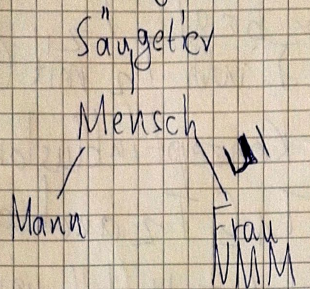
\includegraphics[width=3.71910in,height=1.83200in]{media/haase.png}


\subsubsection{Klassifikation}

Ein weiteres Schlussforlgerungsproblem:

\begin{itemize}
  \item \textbf{Klassifikation}: Gegeben $\MT$, berechne das Hasse Diagramm für $\sqsubseteq$ bzgl. $\MT$, eingeschränkt auf Konzeptnamen in $\MT$.
\end{itemize}

Dies ist ein Berechnungsproblem (kein Entscheidungsproblem), das in der Praxis durch $n^2$ Subsumtionsberchnungen berechenbar ist und für das zahlreiche Optimierungen verfügbar sind.

\subsubsection{Reduktion}

Die Entscheidungsprobleme sind wechselseitig polynomiell aufeinander reduzierbar:

\begin{lemma}
\begin{enumerate}
\item{\emph{Erfüllbarkeit} auf \emph{Nicht-Äquivalenz} \\
$C$ erfüllbar bzgl. $\MT$ gdw. $T \not\vDash C \equiv \bot$}
\item{\emph{Subsumtion} auf \emph{Unerfüllbarkeit} \\
$T \vDash C \sqsubseteq D$ gdw. $C \sqcap \neg D$ unerfüllbar bzgl.
$\MT$
\item{\emph{Äquivalenz} auf \emph{Subsumtion} \\}
$T \vDash C \equiv D$ \emph{gdw.} $T \vDash \top \sqsubseteq \left( C \sqcap D \right) \sqcup \left( \neg C \sqcap \neg D \right)$}
\end{enumerate}
\end{lemma}

Dies heißt für uns, dass ein Algorithmus für eines der Probleme auch für die anderen beiden verwendet werden können. Alle drei Probleme haben dieselbe Komplexität (in $\ALC$). Daher werden wir uns im Folgenden hauptsächlich auch Erfüllbarkeit konzentrieren.

\subsection{Erweiterungen von $\ALC$}\label{erweiterungen-von-alc}

Wir betrachten exemplarisch die beiden Erweiterungen $\ALCI$ und $\ALCQ$ von $\ALC$. Es existieren viel mehr Erweiterungen (z.B.: um spezielle Rolleniterpretationen, temporale Operatoren etc.). Diese können auch kombiniert werden, z.B.: $\ALCQI$.

\subsubsection{Inverse Rollen ($\ALCI$)}\label{inverse-rollen-alci}

Zunächst betrachten wir $\ALCI$, das $\ALC$ um die Möglichkeit inverse Rollen in Existenz- und Werterestriktionen zu benutzen erweitert.

\begin{definition}{Inverse Rollen}
Für jeden Rollennamen $r$ ist $r^{-}$ die \emph{inverse
Rolle} zu $r$. Wir definieren \\
$\left( r^{-} \right)^{\MI} = \left\{ \left( e,d \right)\  \right|\ \left( d,e \right) \in r^{\MI}\}$
\end{definition}

\subsubsection{Zahlenrestriktion ($\ALCQ$)}\label{zahlenrestriktion-alcq}

\begin{definition}{Zahlenrestriktion}
Für jede natürliche Zahl $n$, jeden Rollennamen $r$ und
jedes Konzept $C$:

\begin{itemize}
  \item $\left( \leq n\ r\ C \right)$ (Höchstens-Restriktion)
  \item $\left( \geq n\ r\ C \right)$ (Mindestens-Restriktion)
\end{itemize}

Die Semantik ist
\begin{itemize}
\item
  Höchstens-Restriktion:
  $\left( \leq n\ r\ C \right)^{\MI} = \left\{ d \in \Delta^{\MI}\ |\ \#\left\{ e\ |\ \left( d,e \right) \in r^{\MI} \land e \in C^{\MI} \right\} \leq n \right\}$
\item
  Mindestens-Restriktion
  $( \geq n\ r\ C) = \left\{ d \in \Delta^{\MI}\ |\ \#\left\{ e\ |\ \left( d,e \right) \in r^{\MI} \land e \in C^{\MI} \right\} \geq n \right\}$
\end{itemize}
\end{definition}

Beachte:

\begin{itemize}
  \item $\exists r.C$ ist äquivalent zu $(\geq 1\ r\ C)$
  \item $\forall r.C$ ist äquivalent zu $(\leq 0\ r\ \neg C)$
\end{itemize}